\index{WCET}

\index{WCET!analysis}

Worst-case execution time (WCET) estimates of tasks are essential for
designing and verifying real-time systems. WCET estimates can be
obtained either by measurement or static analysis. The problem with
using measurements is that the execution times of tasks tend to be
sensitive to their inputs. As a rule, measurement does not guarantee
safe WCET estimates. Instead, static analysis is necessary for hard
real-time systems. Static analysis is usually divided into a number
of different phases:
\begin{description}
    \item[Path analysis] generates the control flow graph (a directed
    graph of basic blocks) of the program and annotates (manual or
    automatic) loops with bounds.
    \item[Low-level analysis] determines the execution time of basic
    blocks obtained by the path analysis. A model of the processor
    and the pipeline provides the execution time for the instruction
    sequence.
    \item[Global low-level analysis] determines the influence of
    hardware features such as caches on program execution time. This
    analysis can use information from the path analysis to provide less
    pessimistic values.
    \item[WCET Calculation] The final WCET is calculated by
        transforming the control flow graph with the timing
        information of basic blocks\footnote{A basic block is a
        sequence of instructions without any jumps or jump
        targets within this sequence.} with the program
        annotations for loops to an integer linear programming
        (ILP) problem. This problem is solved by an ILP solver.
        This approach is also called implicit path enumeration
        (IPET).
\end{description}

For the low-level analysis, a good timing model of the processor is
needed. The main problem for the low-level analysis is the execution
time dependency of instructions in modern processors that are not
designed for real-time systems. JOP is designed to be an easy target
for WCET analysis. The WCET of each bytecode can be predicted in
terms of the number of cycles it requires. There are no timing
dependencies between bytecodes.

WCET analysis has to be done at two levels: at the microcode level
and at the bytecode level. The microcode WCET analysis is performed
only once for a processor configuration and described in the next
section. The result from this microcode analysis is the timing model
of the  processor. The timing model is the input for WCET analysis at
the bytecode level (i.e.\ the Java application) as explained in
Section~\ref{sec:wcet:app}.

The first WCET analysis tool that targets JOP has been developed by
Rasmus Pedersen \cite{jop:wcet:jtres06}. Benedikt Huber implemented a
new version of the analyzer with support of bytecodes implemented in
Java and a better method cache approximation has
\cite{jop:wcet:model:checking}. The new tool also contains a module
to extract the low-level bytecode timing from the microcode assembler
program (\code{jvm.asm}) automatically.

\section{Microcode WCET Analysis}
\index{WCET!microcode}

Each bytecode is implemented by microcode. We can obtain the WCET of
a single bytecode by performing WCET analysis at the microcode level.
To prove that there are no time dependencies between bytecodes, we
have to show that no processor states are \emph{shared} between
different bytecodes.

\subsection{Microcode Path Analysis}

To obtain the WCET values for the individual bytecodes we perform
the path analysis at the microcode level. First, we have to ensure
that a number of restrictions (from \cite{pusch:maxt:jnl}) of the
code are fulfilled:
%
\begin{itemize}
    \item Programs must not contain unbounded recursion. This property
    is satisfied by the fact that there exists no call instruction in
    microcode.
    \item Function pointers and computed \code{gotos} complicate the
    path analysis and should therefore be avoided. Only simple conditional
    branches are available at the microcode level.
    \item The upper bound of each loop has to be known. This is the only
    point that has to be verified by inspection of the microcode.
\end{itemize}
%
To detect loops in the microcode we have to find all backward
branches (e.g.\ with a negative branch offset).\footnote{The loop
branch can be a forward branch. However, the basic blocks of the loop
contain at least one backward branch. Therefore we can identify all
loops by searching for backward branches only.} The branch offsets
can be found in a VHDL file (\code{offtbl.vhd}) that is generated
during microcode assembly. In the current implementation of the JVM
there are ten different negative offsets. However, not each offset
represents a loop. Most of these branches are used to share common
code. Three branches are found in the initialization code of the JVM.
They are not part of a bytecode implementation and can be ignored.
The only loop that is found in a regular bytecode is in the
implementation of \code{imul} to perform a fixed delay. The iteration
count for this loop is constant.

A few bytecodes are implemented in Java\footnote{The implementation
can be found in the class \code{com.jopdesign.sys.JVM}.} and can be
analyzed in the same way as application code. The bytecodes
\code{idiv} and \code{irem} contain a constant loop. The bytecode
\code{lookupswitch}\footnote{\codefoot{lookupswitch} is one way of
implementing the Java \codefoot{switch} statement. The other
bytecode, \codefoot{tableswitch}, uses an index in the table of
branch offsets and has therefore a constant execution time.} performs
a linear search through a table of branch offsets. The WCET depends
on the table size that can be found as part of the instruction.

As the microcode sequences are very short, the calculation of the
control flow graph for each bytecode is done manually.

\subsection{Microcode Low-level Analysis}

To calculate the execution time of basic blocks in the microcode, we
need to establish the timing of microcode instructions on JOP. All
microcode instructions except \code{wait} execute in a single cycle,
reducing the low-level analysis to a case of merely counting the
instructions.

The \code{wait} instruction is used to stall the processor and wait
for the memory subsystem to finish a memory transaction. The
execution time of the \code{wait} instruction depends on the memory
system and, if the memory system is predictable, has a known WCET. A
main memory consisting of SRAM chips can provide this predictability
and this solution is therefore advised. The predictable handling of
DMA, which is used for the instruction cache fill, is explained in
Section~\ref{sec:cache}. The \code{wait} instruction is the only way
to stall the processor. Hardware events, such as interrupts (see
Section~\ref{sec:interrupt}), do not stall the processor.

Microcode is stored in on-chip memory with single cycle access. Each
microcode instruction is a single word long and there is no need for
either caching or prefetching at this stage. We can therefore omit
the low-level analysis. No pipeline analysis \cite{EngblomPhD}, with
its possible unbounded timing effects, is necessary.

\subsection{Bytecode Independency}

We have seen that all microcode instructions except \code{wait} take
one cycle to execute and are therefore independent of other
instructions. This property directly translates to independency of
bytecode instructions.

The \code{wait} microcode instruction provides a convenient way to
hide memory access time. A memory read or write can be triggered in
microcode and the processor can continue with microcode
instructions. When the data from a memory read is needed, the
processor explicitly waits, with the \code{wait} instruction, until
it becomes available.

For a memory store, this \code{wait} could be deferred until the
memory system is used next (similar to a write buffer). It is
possible to initiate the store in a bytecode such as \code{putfield}
and continue with the execution of the next bytecode, even when the
store has not been completed. In this case, we introduce a
dependency over bytecode boundaries, as the state of the memory
system is \emph{shared}. To avoid these dependencies that are
difficult to analyze, each bytecode that accesses memory waits
(preferably at the end of the microcode sequence) for the completion
of the memory request.

Furthermore, if we would not wait at the end of the store operation
we would have to insert an additional \code{wait} at the start of
every read operation. Since read operations are more frequent than
write operations (15\% vs. 2.5\%, see \cite{jop:thesis}), the
performance gain from the hidden memory store is lost.

\subsection{WCET of Bytecodes}
\index{WCET!bytecode timing} \index{bytecode!execution time}

\label{sec:wcet:bc} The control flow of the individual bytecodes
together with the basic block length (that directly corresponds with
the execution time) and the time for memory access result in the WCET
(and BCET) values of the bytecodes. These values can be found in
Appendix~\ref{appx:bytecode}.

\subsubsection{Basic Bytecodes}

Most bytecode instructions that do not access memory have a constant
execution time. They are executed by either one microcode instruction
or a short sequence of microcode instructions. The execution time in
clock cycles equals the number of microinstructions executed. As the
stack is on-chip, it can be accessed in a single cycle. We do not
need to incorporate the main memory timing into the instruction
timing. Most simple bytecodes execute in a single cycle.
Table~\ref{tab:simple} shows example instructions, their timing, and
their meaning. Access to object, array, and class fields depend on
the timing of the main memory.

\begin{table}
\centering
\begin{tabular}{rlcl}
    \toprule
    Opcode & Instruction & Cycles & Funtion\\
    \midrule
3 & iconst\_0  & 1 & load constant 0 on TOS\\
4 & iconst\_1  & 1 & load constant 1 on TOS\\
16 & bipush & 2 & load a byte constant on TOS\\
17 & sipush & 3 & load a short constant on TOS\\
21 & iload  & 2 & load a local on TOS\\
26 & iload\_0 & 1 & load local 0 on TOS\\
27 & iload\_1 & 1 & load local 1 on TOS\\
54 & istore  & 2 & store the TOS in a local\\
59 & istore\_0 & 1 & store the TOS in local 0\\
60 & istore\_1 & 1 & store the TOS in local 1\\
89 & dup & 1 & duplicate TOS\\
90 & dup\_x1 & 5 & complex stack manipulation\\
96 & iadd & 1 & integer addition\\
153 & ifeq & 4 & conditional branch\\
    \bottomrule
\end{tabular}
    \caption{Execution time of simple bytecodes in cycles}
    \label{tab:simple}
\end{table}


\subsubsection{Object Oriented Bytecodes}
\index{WCET!memory access}

Object oriented instructions, array access, and invoke instructions
access the main memory. Therefore, we have to model the memory access
time. We assume a simple SRAM with a constant access time. Access
time that exceeds a single cycle includes additional wait states
($r_{ws}$ for a memory read and $w_{ws}$ for a memory write). With a
memory with $r_{ws}$ wait states, the execution time for, e.g.,
\code{getfield} is
\begin{equation*}
    t_{\textit{getfield}} = 11 + 2 r_{ws}
\end{equation*}

The memory subsystem performs reads and writes in parallel to the
execution of microcode. Therefore, some access cycles can be hidden.
The following example gives the exact execution time of bytecode
\code{ldc2\_w} in clock cycles:
%
\begin{equation*}
    t_{ldc2\_w} = 17+\left\{\begin{array}{r@{\quad:\quad}l}
    r_{ws}-2 & r_{ws}>2 \\
    0   & r_{ws}\le2
    \end{array} \right.
    +
    \left\{\begin{array}{r@{\quad:\quad}l}
    r_{ws}-1 & r_{ws}>1 \\
    0   & r_{ws}\le1
    \end{array} \right.
\end{equation*}
%
Thus, for a memory with two cycles access time ($r_{ws}=1)$, as we
use it for a 100~MHz version of JOP with a 15~ns SRAM, the wait state
is completely hidden by microcode instructions for this bytecode.

Memory access time also determines the cache load time on a miss. For
the current implementation the cache load time is calculated as
follows: the wait state $c_{ws}$ for a single word cache load is:
\begin{equation*}
    c_{ws} =
    \left\{\begin{array}{r@{\quad:\quad}l}
    r_{ws} & r_{ws}>1 \\
    1   & r_{ws}\le1
    \end{array} \right.
\end{equation*}
%
On a method invoke or return, the respective method has to be loaded
into the cache on a cache miss. The load time $l$ is:
\index{cache!load time}
%
\[
    l =
    \left\{\begin{array}{r@{\quad:\quad}l}
    6+(n+1)(1+c_{ws}) & \mbox{cache miss} \\
    4   & \mbox{cache hit}
    \end{array} \right.
\]
where $n$ is the size of the method in number of 32-bit words. For
short methods, the load time of the method on a cache miss, or part
of it, is hidden by microcode execution. As an example, the exact
execution time for the bytecode \code{invokestatic} is:
%
\begin{equation*}
    t = 74+r_{ws}+
    \left\{\begin{array}{r@{\quad:\quad}l}
    r_{ws}-3 & r_{ws}>3 \\
    0   & r_{ws}\le3
    \end{array} \right.
    +
    \left\{\begin{array}{r@{\quad:\quad}l}
    r_{ws}-2 & r_{ws}>2 \\
    4   & r_{ws}\le2
    \end{array} \right.
    +
    \left\{\begin{array}{r@{\quad:\quad}l}
    l-37 & l>37 \\
    0   & l\le37
    \end{array} \right.
\end{equation*}
%

For \code{invokestatic} a cache load time $l$ of up to 37 cycles is
completely hidden. For the example SRAM timing the cache load of
methods up to 36 bytes long is hidden. The WCET analysis tool, as
described in the next section, knows the length of the invoked method
and can therefore calculate the time for the invoke instruction cycle
accurate.

\subsubsection{Bytecodes in Java}

Bytecodes can be implemented in Java on JOP. In this case, a static
method from a JVM internal class gets invoked when such a bytecode is
executed. For WCET analysis this bytecode is substituted by an invoke
instruction to this method. The influence on the cache (the bytecode
execution results in a method load) can be analyzed in the same way
as for \emph{ordinary} static methods.

%\begin{itemize}
%    \item Java based bytecodes -- handle them as methods
%    \item \code{new} with constant execution time (in our current GC
%    implementation and also possible with scopes)
%\end{itemize}

\subsubsection{Native Methods}

Most of the JVM internal functionality in JOP, such as input, output,
and thread scheduling, is implemented in Java. However, Java and the
JVM do not allow direct access to memory, peripheral devices or
processor registers. For this low-level access to system resources,
we need \emph{native} methods. For a Java processor, the
\emph{native} language is still Java bytecode. We solve this issue by
substituting the native method invocation by a special bytecode
instruction on class loading. Those special bytecodes are implemented
in JOP microcode in the same way as regular bytecodes (see
Section~\ref{sec:microcode}. The execution time of the native methods
(or in other words special bytecodes) is given in the same way as the
execution time for standard bytecodes.

\section{WCET Analysis of the Java Application}
\label{sec:wcet:app} \index{WCET!analysis}

In hard real-time systems, the estimation of the worst-case execution
time (WCET) is essential. WCET analysis is in general an undecidable
problem. Program restrictions, as given in \cite{pusch:maxt:jnl},
make this problem decidable:
\begin{enumerate}
    \item Programs must not contain any recursion
    \item Absence of function pointers
    \item The upper bound of each loop has to be known
\end{enumerate}
Recursive algorithms have to be transformed to iterative ones. For
our WCET analyzer, the loop bounds are detected by data-flow analysis
or have to be annotated in the program source. However, we want to
relax the second restriction regarding function pointers. Function
pointers are similar to inherited or overridden methods: they are
dispatched at runtime. For an object-oriented language this mechanism
is fundamental. In contrast to function pointers, e.g., in C, we can
statically analyze which methods can be invoked when the whole
program is known. Therefore, we allow dynamic dispatching of methods
in Java in our analysis.

We replace the function pointer restriction by the following
restriction: \emph{Dynamic class loading is not allowed}. As the full
application has to be available for WCET analysis, dynamic class
loading cannot be supported. For embedded real-time systems this is
not a severe restriction.

\subsection{High-Level WCET Analysis}

The high-level WCET analysis, presented in this section, is based on
standard technologies \cite{Puschner:JRTS1997, 216666}. From the
class files that make up the application, the relevant information is
extracted. The CFG of the basic blocks is extracted from the
bytecodes. Annotations for the loop counts are either provided by the
data-flow analysis or are extracted from comments in the source.
Furthermore, the class hierarchy is examined to find all possible
targets for a method invoke and the data-flow analysis tightens the
set of possible receivers.

Java bytecode generation has to follow stringent rules \cite{jvm} in
order to pass the class file verification of the JVM. Those
restrictions lead to an \emph{analysis friendly} code; e.g. the stack
size is known at each instruction. The control flow instructions are
well defined. Branches are relative and the destination is within the
same method. In the normal program, there is no instruction that
loads a branch destination in a local variable or onto the
stack.\footnote{The exception are bytecodes \codefoot{jsr} and
\codefoot{ret} that use the stack and a local variable for the return
address of a method local subroutine. This construct can be used to
implement the \codefoot{finally} clauses of the Java programming
language. However, this problematic subroutine can be easily inlined
\cite{gc:subroutine:inlining}. Furthermore, Sun's Java compilers
version 1.4.2 and later compile \codefoot{finally} blocks without
subroutines.} Detection of basic blocks in Java bytecode and
construction of the CFG is thus straight forward.

In Java class files there is more information available than in
compiled C/C++ executables. All links are symbolic and it is possible
to reconstruct the class hierarchy from the class files. Therefore,
we can statically determine all possible targets for a virtual method
invoke.

WCET analysis at the bytecode level has several advantages when the
execution time of the individual bytecodes are known. When compiled
with debug information references to the source are stored in the
class file. With this information it is possible to extract
annotations in the Java source code. We use this feature to annotated
loop bounds within comments in the Java source. This form of
annotation is simple and less intrusive than using a predefined dummy
class as suggested in \cite{R:Bernat:2000a}.

\subsection{WCET Annotations} \label{sec:annot}
\index{WCET!annotations}

Simple loop bounds are detected by the data-flow analysis
\cite{dfa:puffitsch:2009}. For cases where the bounds are not
detectable, we additionally support annotations in the source. The
annotations are written as comments (see
Listing~\ref{lst:wcet:example}). It would be more convenient to use
standard Java annotations introduced with Java 1.5, as they are
checked at compile time. However, at the moment Java annotations are
not allowed at code block level. A proposal to remove this
restriction is currently under review (JSR 308). When compiling Java,
the source line information is included in the class file. Therefore,
when a loop is detected in the CFG, the relevant source line for the
loop header is looked up in the source and the annotation is
extracted from the comment.

Annotations given as source comments are simple and less intrusive
than using a predefined dummy class \cite{R:Bernat:2000a}. Two
variants of the loop bounding annotation are supported: one with an
exact bound\footnote{The exact bound has been used to find best-case
values for some test settings.} ($=$) and one that places an upper
bound on the iterations ($<=$). The extension to more elaborate
annotations, as suggested in \cite{pusch:maxt:jnl} and
\cite{R:Bernat:2000a}, can provide even tighter WCET bounds.

%Both types are shown in Figure \ref{fig:annotation}. The two
%variants enable both BCET and WCET execution time analysis.

\subsection{ILP Formulation} \label{sec:ilp}
\index{WCET!integer linear programming}

The calculation of the WCET is transformed to an ILP problem
\cite{Puschner:JRTS1997}. In the CFG, each vertex represents a basic
block $B_i$ with execution time $c_i$. With the basic block execution
frequency $e_i$ the WCET is:
\begin{equation*}
    WCET = max\sum_{i=1}^{N}c_i e_i
\end{equation*}
The sum is the objective function for the ILP problem. The maximum
value of this expression results in the WCET of the program.

Furthermore, each edge is also assigned an execution frequency $f$.
These execution frequencies represent the control flow through the
WCET path. Two primary constraints form the ILP problem: (i) For each
vertex, the sum of $f_j$ for the incoming edges has to be equal to
the sum of the $f_k$ of the outgoing edges; (ii) The frequency of the
edges connecting the loop body with the loop header, is less than or
equal to the frequency of the edges entering the loop multiplied by
the loop bound.

% (ii) The frequency of one
% edge in the loop $f_l$, e.g., the edge entering the loop body, is
% equal or less than the frequency $f_h$ of the edges into the loop
% header multiplied by the loop bound.
% bhu: The old version is not quite correct: 'into the loop header'
% includes the backedge but must not, and one should also allow more
% than one backedge.

From the CFG, which represents the program structure, we can extract
the flow constraints. With the execution frequency $f$ of the edges
and the two sets $I_i$ for the incoming edges to basic block $B_i$
and $O_i$ for the outgoing edges, the execution frequency $e_i$ of
$B_i$ is:
\begin{equation*}
    e_i = \sum_{j\in I_i} f_j = \sum_{k\in O_i} f_k
\end{equation*}
The frequencies $f$ are the integer variables calculated by solving
the ILP problem. Furthermore, we add two special vertices to the
graph: The start node $S$ and the termination node $T$. The start
node $S$ has only one outgoing edge that points to the first basic
block of the program. The execution frequency $f_s$ of this edge is
set to 1. The termination node $T$ has only incoming edges with the
sum of the frequencies also set to 1; all return statements of a
method are connected to the node $T$. This means that the program is
executed once and can only terminate once through $T$.

Loop bounds are additional constraints for the ILP problem. A special
vertex, the loop header, is connected by following edges:
\begin{enumerate}
    \item Incoming edges that enter the loop with frequency $f_h$
    \item One outgoing edge entering the loop body with frequency
        $f_l$
    \item Incoming edges that close the loop
    \item One loop exit edge
\end{enumerate}
With the maximum loop count (the loop bound) $n$ we formulate the
loop constraint as
\begin{equation*}
    f_l \le n \sum f_h
\end{equation*}
This explanation is a little bit simplified, as more complex loop
conditions have several edges to the loop body. Therefore, the tool
considers the set of incoming edges to the loop header that close the
loop for the ILP constraint.

Without further global constraints the problem can be solved locally
for each method. We start at the leaves of the call tree and
calculate the WCET for each method. The WCET value of a method is
included in the invoke instruction of the caller method. To
incorporate global constraints, such as cache constraints
\cite{828940}, a single CFG is built that contains the whole program
by inserting edges from the invoke instruction to the invoked method
and back. This is conceptually equivalent to inlining each method.

In Section~\ref{sec:wcet:cache}, we will show how the cache
constraints for the method cache can be integrated into the analysis.
%A simplified version to classify method invocations as single miss when
%all invoked methods in a loop will fit into the cache, can be easily
%integrated into the ILP constraints.



\begin{lstlisting}[float=t, caption={The example used for WCET analysis},label=lst:wcet:example]

public static int loop(boolean b, int val) {

    int i, j;

    for (i=0; i<10; ++i) {          // @WCA loop=10
        if (b) {
            for (j=0; j<3; ++j) {   // @WCA loop=3
                val *= val;
            }
        } else {
            for (j=0; j<4; ++j) {   // @WCA loop=4
                val += val;
            }
        }
    }
    return val;
}
\end{lstlisting}

\subsection{An Example}

To illustrate the WCET analysis flow we provide a small example.
Listing~\ref{lst:wcet:example} shows the Java source code that
contains nested loops with a condition. The simple loop bounds are
detected by the data-flow analysis (DFA). We just show in the example
how the annotation syntax looks like. In our target hardware, the
multiplication takes longer than the addition. Therefore, in this
example, it is not obvious which branch will result in the WCET path.

Table~\ref{tab:wcet:bytecode} shows the bytecodes and basic blocks of
the example, as generated by our WCET analysis tool. The fourth
column gives the execution time of the bytecodes in clock cycles. The
fifth column gives the execution time of the basic blocks. These are
the values used for the ILP equations.

\begin{figure}[t]
    \centering
    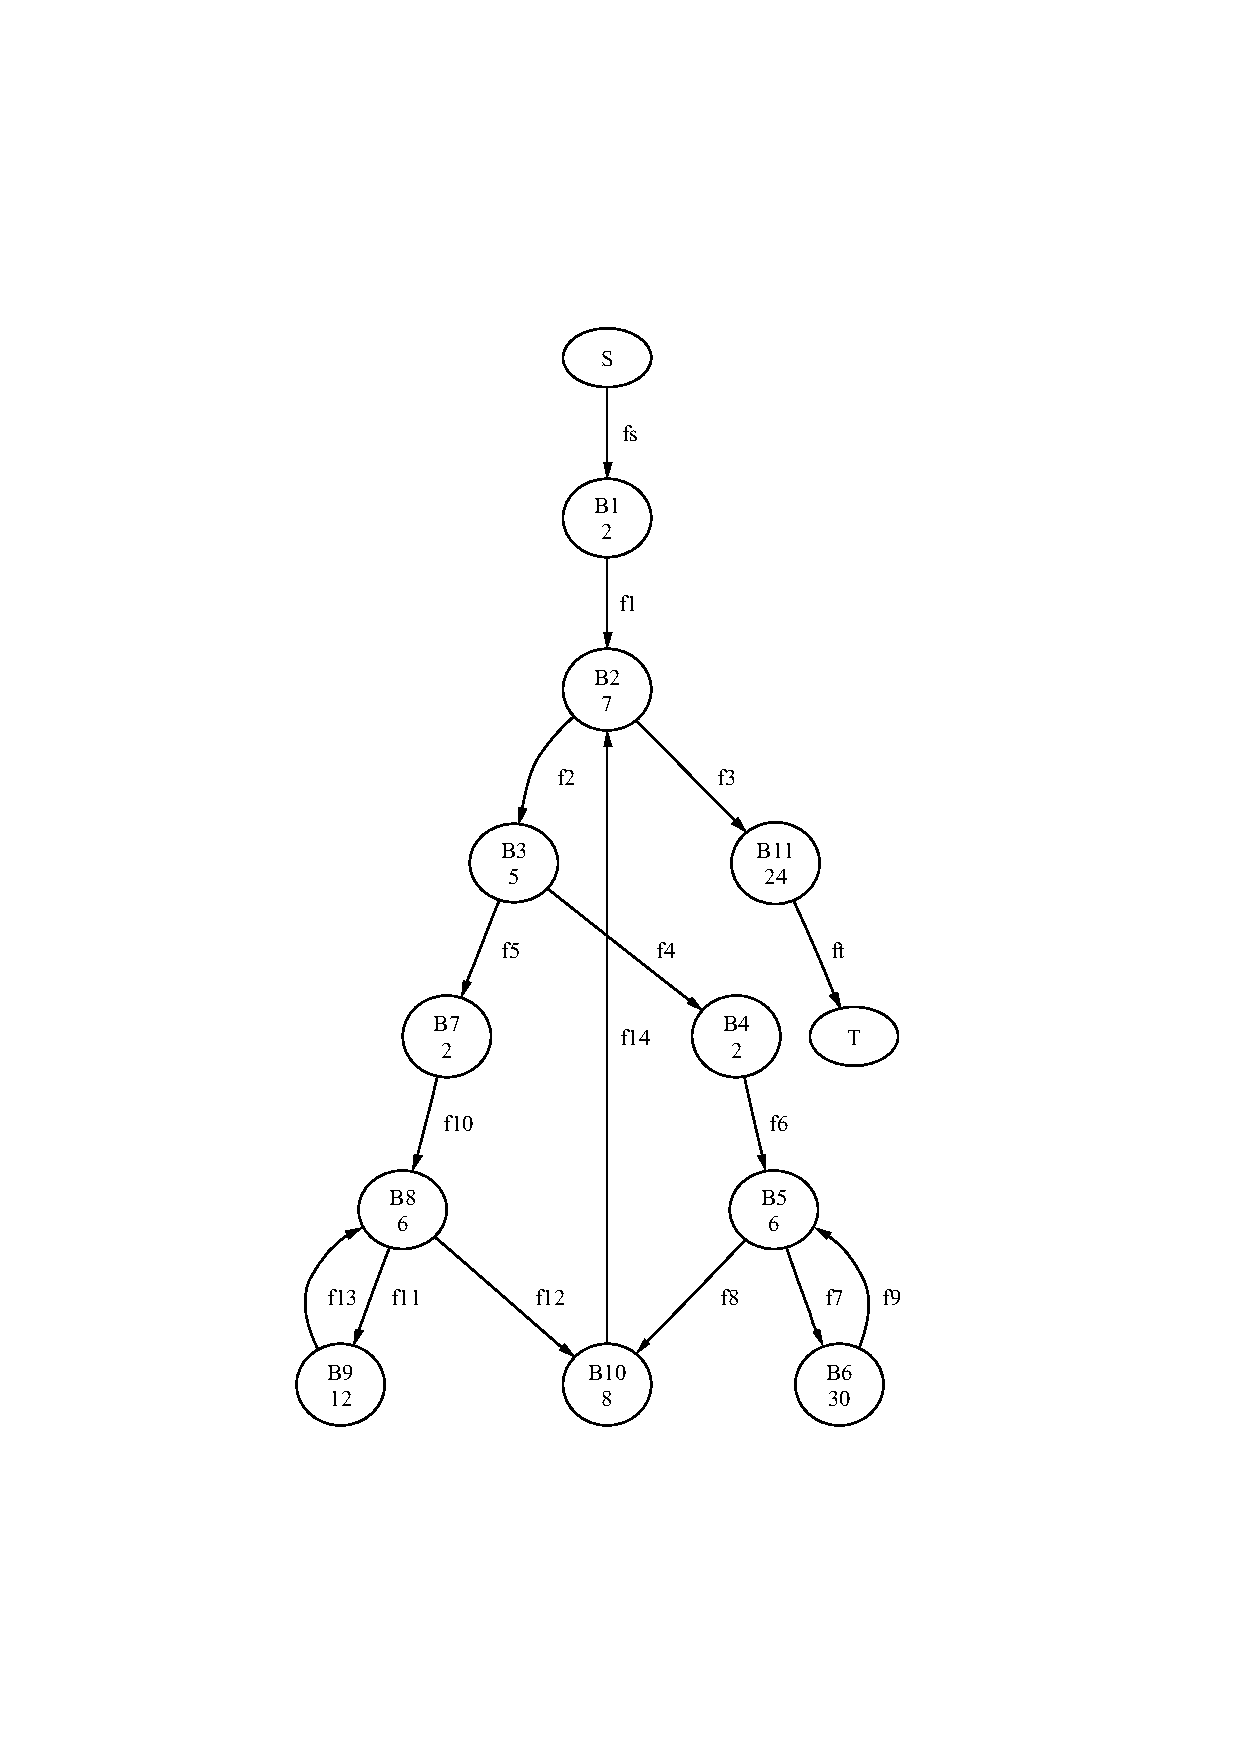
\includegraphics[scale=0.5]{wcet/loop}
    \caption{CFG of the example}
    \label{fig:cfg}
\end{figure}



\begin{table}
\begin{center}
\begin{tiny}
\begin{tabular}{lllrr}
    \toprule
    Block & Addr. & Bytecode & Cycles & BB Cycles\\
    \midrule
B1  & 0: &     iconst\_0         &           1        &           \\
    & 1: &     istore\_2         &           1        &                2 \\
    \cmidrule{1-5}
B2  & 2: &     iload\_2          &           1        &           \\
    & 3: &     bipush            &          2         &          \\
    & 5: &     if\_icmpge 55     &           4        &                7 \\
    \cmidrule{1-5}
B3  & 8: &     iload\_0          &           1        &           \\
    & 9: &     ifeq 30           &          4         &               5 \\
    \cmidrule{1-5}
B4  & 12: &    iconst\_0         &           1        &           \\
    & 13: &    istore\_3         &           1        &                2 \\
    \cmidrule{1-5}
B5  & 14: &    iload\_3          &           1        &           \\
    & 15: &    iconst\_3         &           1        &           \\
    & 16: &    if\_icmpge 48     &           4        &                6 \\
    \cmidrule{1-5}
B6  & 19: &    iload\_1          &           1        &           \\
    & 20: &    iload\_1          &           1        &           \\
    & 21: &    imul              &         19         &          \\
    & 22: &    istore\_1         &           1        &           \\
    & 23: &    iload\_3          &           1        &           \\
    & 24: &    iconst\_1         &           1        &           \\
    & 25: &    iadd              &          1         &          \\
    & 26: &    istore\_3         &           1        &           \\
    & 27: &    goto 14           &          4         &              30 \\
    \cmidrule{1-5}
B7  & 30: &    iconst\_0         &           1        &           \\
    & 31: &    istore\_3         &           1        &                2 \\
    \cmidrule{1-5}
B8  & 32: &    iload\_3          &           1        &           \\
    & 33: &    iconst\_4         &           1        &           \\
    & 34: &    if\_icmpge 48     &           4        &                6 \\
    \cmidrule{1-5}
B9  & 37: &    iload\_1          &           1        &           \\
    & 38: &    iload\_1          &           1        &           \\
    & 39: &    iadd              &          1         &          \\
    & 40: &    istore\_1         &           1        &           \\
    & 41: &    iload\_3          &           1        &           \\
    & 42: &    iconst\_1         &           1        &           \\
    & 43: &    iadd              &          1         &          \\
    & 44: &    istore\_3         &           1        &           \\
    & 45: &    goto 32           &          4         &              12 \\
    \cmidrule{1-5}
B10 & 48: &    iload\_2          &           1        &           \\
    & 49: &    iconst\_1         &           1        &           \\
    & 50: &    iadd              &          1         &          \\
    & 51: &    istore\_2         &           1        &           \\
    & 52: &    goto 2            &          4         &               8 \\
    \cmidrule{1-5}
B11 & 55: &    iload\_1          &           1        &           \\
    & 56: &    ireturn           &         23         &              24 \\
    \bottomrule
\end{tabular}
\end{tiny}
\end{center}
    \caption{Java bytecode and basic blocks}
    \label{tab:wcet:bytecode}
\end{table}

From the basic blocks, we can construct the CFG as shown in
Figure~\ref{fig:cfg}. The vertices represent the basic blocks and
include the execution time in clock cycles. We can identify block B2
as the loop header for the outer loop. B3 is the branch node. B5 and
B8 are the loop headers for the inner loops.


From the CFG, we can extract the flow constraints by the following
fact: The execution frequency of a basic block is equal to the
execution frequency of all incoming edges and equal to the execution
frequency of all outgoing edges. E.g.,\ for block B2 the execution
frequency $e_2$ is:
\begin{equation*}
    e_2 = f_{1} + f_{14} = f_{2} + f_{3}
\end{equation*}

%With execution time $c_i$ and execution frequency $e_i$ of basic
%block $B_i$ the WCET is the maximum value of
%\begin{equation*}
%    \sum_{i=1}^{N}c_i e_i
%\end{equation*}
%This is also our objective function for the ILP problem.

The loop constraints are formulated by constraining the frequency of
the loop's back edges. The loop bounds are automatically transferred
from the DFA module or extracted from the source annotations. For the
outer loop in the example this is:
% bhu: @rup: I fixed this (f2->f14) to match the actual implementation,
% which also works if there is a compound loop condition like (a && b)
\begin{equation*}
    f_{14} = 10 f_1
\end{equation*}


In Listing~\ref{lst:ilp}, the resulting equations for the integer
linear programming problem, as generated by our tool, are listed. We
use the open-source ILP solver
\code{lp\_solve}.\footnote{\url{http://lpsolve.sourceforge.net/5.5/}}

\index{WCET!ILP example}

\begin{lstlisting}[float, caption={ILP equations of the example},label=lst:ilp]

    /* Objective function */
    max: t1 t2 t3 t4 t5 t6 t7 t8 t9 t10 t11;
    /* flow constraints */
    S:  fs = 1;
    B1: fs = f1;
    B2: f14 + f1 = f2 + f3;
    B3: f2 = f4 + f5;
    B4: f4 = f6;
    B5: f9 + f6 = f7 + f8;
    B6: f7 = f9;
    B7: f5 = f10;
    B8: f10 + f13 = f11 + f12;
    B9: f11 = f13;
    B10: f12 + f8 = f14;
    B11: f3 = ft;
    T: ft = 1;
    /* loop bounds */
    f14 = 10 f1;
    f9 = 3 f6;
    f13 = 4 f10;
    /* execution time (with incoming edges) */
    t1 = 2 fs;
    t2 = 7 f14 + 7 f1;
    t3 = 5 f2;
    t4 = 2 f4;
    t5 = 6 f9 + 6 f6;
    t6 = 30 f7;
    t7 = 2 f5;
    t8 = 6 f10 + 6 f13;
    t9 = 12 f11;
    t10 = 8 f12 + 8 f8;
    t11 = 24 f3;
\end{lstlisting}

The ILP solver \code{lp\_solve} gives a result of 1393 cycles. We run
this example on the Java processor for verification. As the execution
time depends only on a single boolean variable, \code{b} (see
Listing~\ref{lst:wcet:example}), it is trivial to measure the actual
WCET. We measure the execution time with a cycle counter for the
execution time of the outer loop, i.e., from the start of block B1
until the exit of the loop at block B2. The last block, B11, which
contains the return statement, is not part of the measurement. The
measured result is 1369 cycles.  When we add the 24 cycles for the
block B11 to our measured WCET, we get 1393 cycles. This measured
result is exactly the same as the analytical result!

\subsection{Dynamic Method Dispatch}

Dynamic runtime-dispatching of inherited or overridden instance
methods is a key feature of object-oriented programming. Therefore,
we allow dynamic methods as a \emph{controlled} form of function
pointers. The full class hierarchy can be extracted from the class
files of the application. From the class hierarchy, we can extract
all possible receiver methods for an invocation. When all possible
receivers are included as alternatives, the resulting WCET bound can
be very pessimistic. Therefore, this set can be tightened by a
flow-sensitive receiver analysis \cite{dfa:puffitsch:2009}.

We include all possible receivers as alternatives in the ILP
constraints. It has to be noted that, without further analysis or
annotations, this can lead to pessimistic WCET estimates.

We split the basic block that contains the invoke instruction into
three new blocks: The preceding instructions, the invoke instruction,
and following instructions. Consider following basic block:

\begin{samepage}
\begin{lstlisting}
    iload_1
    iload_2
    aload_0
    invokevirtual foo
    istore_3
\end{lstlisting}
\end{samepage}

When different versions of \code{foo()} are possible receiver
methods, we model the invocation of \code{foo()} as alternatives in
the graph. The example for two classes \code{A} and \code{B} that are
part of the same hierarchy is shown in
Figure~\ref{fig:dispatch:split}. Following the standard rules for the
incoming and outgoing edges the resulting ILP constraint for this
example is:
\begin{equation*}
    f_1 = f_2 + f_3
\end{equation*}


\begin{figure}
    \centering
    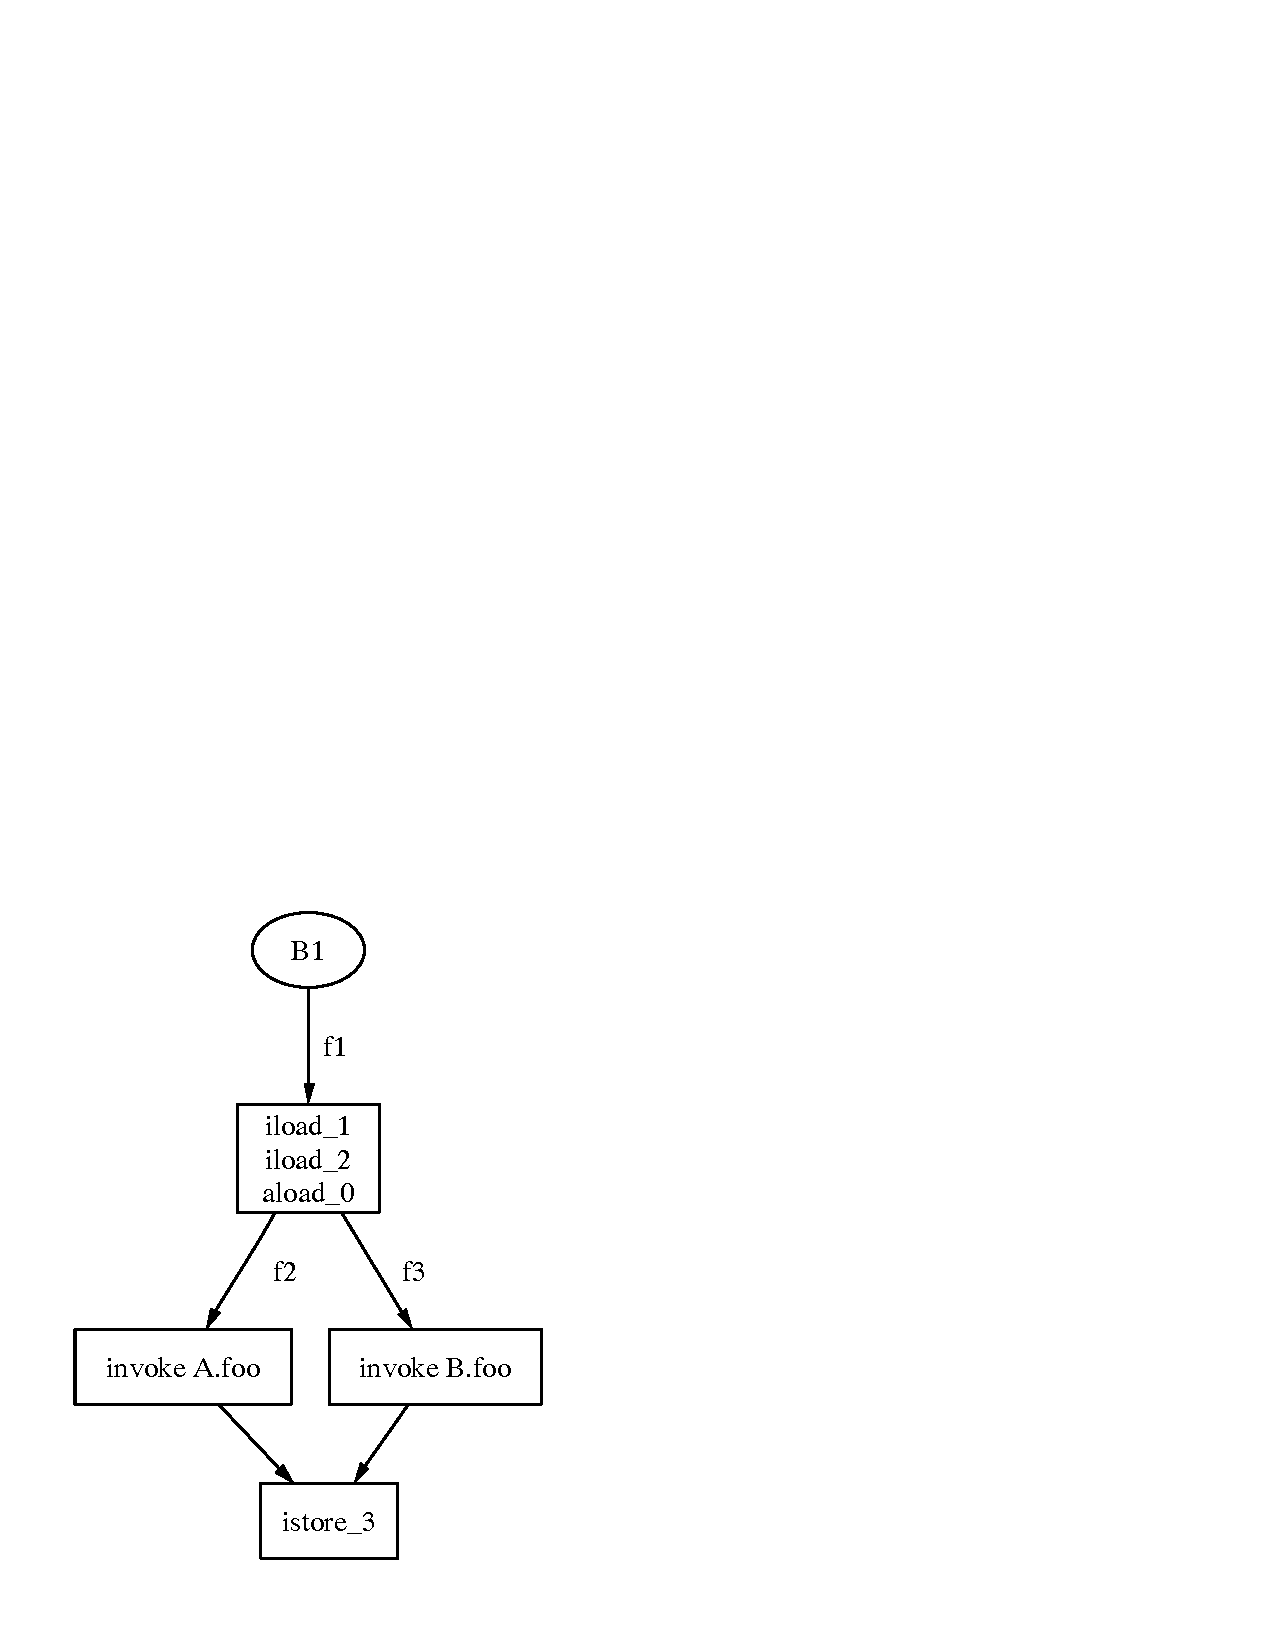
\includegraphics[scale=0.5]{wcet/dispatch_split}
    \caption{Split of the basic block for instance methods}
    \label{fig:dispatch:split}
\end{figure}



\subsection{Cache Analysis} \label{sec:wcet:cache}
\index{WCET!cache analysis}

From the properties of the Java language
--- usually small methods and relative branches --- we derived the
novel idea of a \emph{method cache} \cite{jop:jtres_cache}, i.e.,\ an
instruction cache organization in which whole methods are loaded into
the cache on method invocation and on the return from a method.

The method cache is designed to simplify WCET analysis. Due to the
fact that all cache misses are only included in two instructions
(\emph{invoke} and \emph{return}), the instruction cache can be
ignored on all other instructions. The time needed to load a complete
method is calculated using the memory properties (latency and
bandwidth) and the size of the method. On an invoke, the size of the
invoked method is used, and on a return, the method size of the
caller.

Integration of the method cache into WCET analysis is straight
forward. As the cache hits or misses can only happen at method
invocation, or return from a method, we can model the miss times as
extra vertices in the graph. Figure~\ref{fig:cache:bb} shows an
example with 6 connected basic blocks. Basic block B4 is shown as a
box and has three incoming edges ($f_1$,$f_2$,$f_3$) and two outgoing
edges ($f_5$,$f_6$). B4 contains the invocation of method
\code{foo()}, surrounded by other instructions. The execution
frequency $e_4$ of block B4 in the example is
\begin{equation*}
    e_4 = f_1+f_2+f_3 = f_5+f_6
\end{equation*}

\begin{figure}
    \centering
    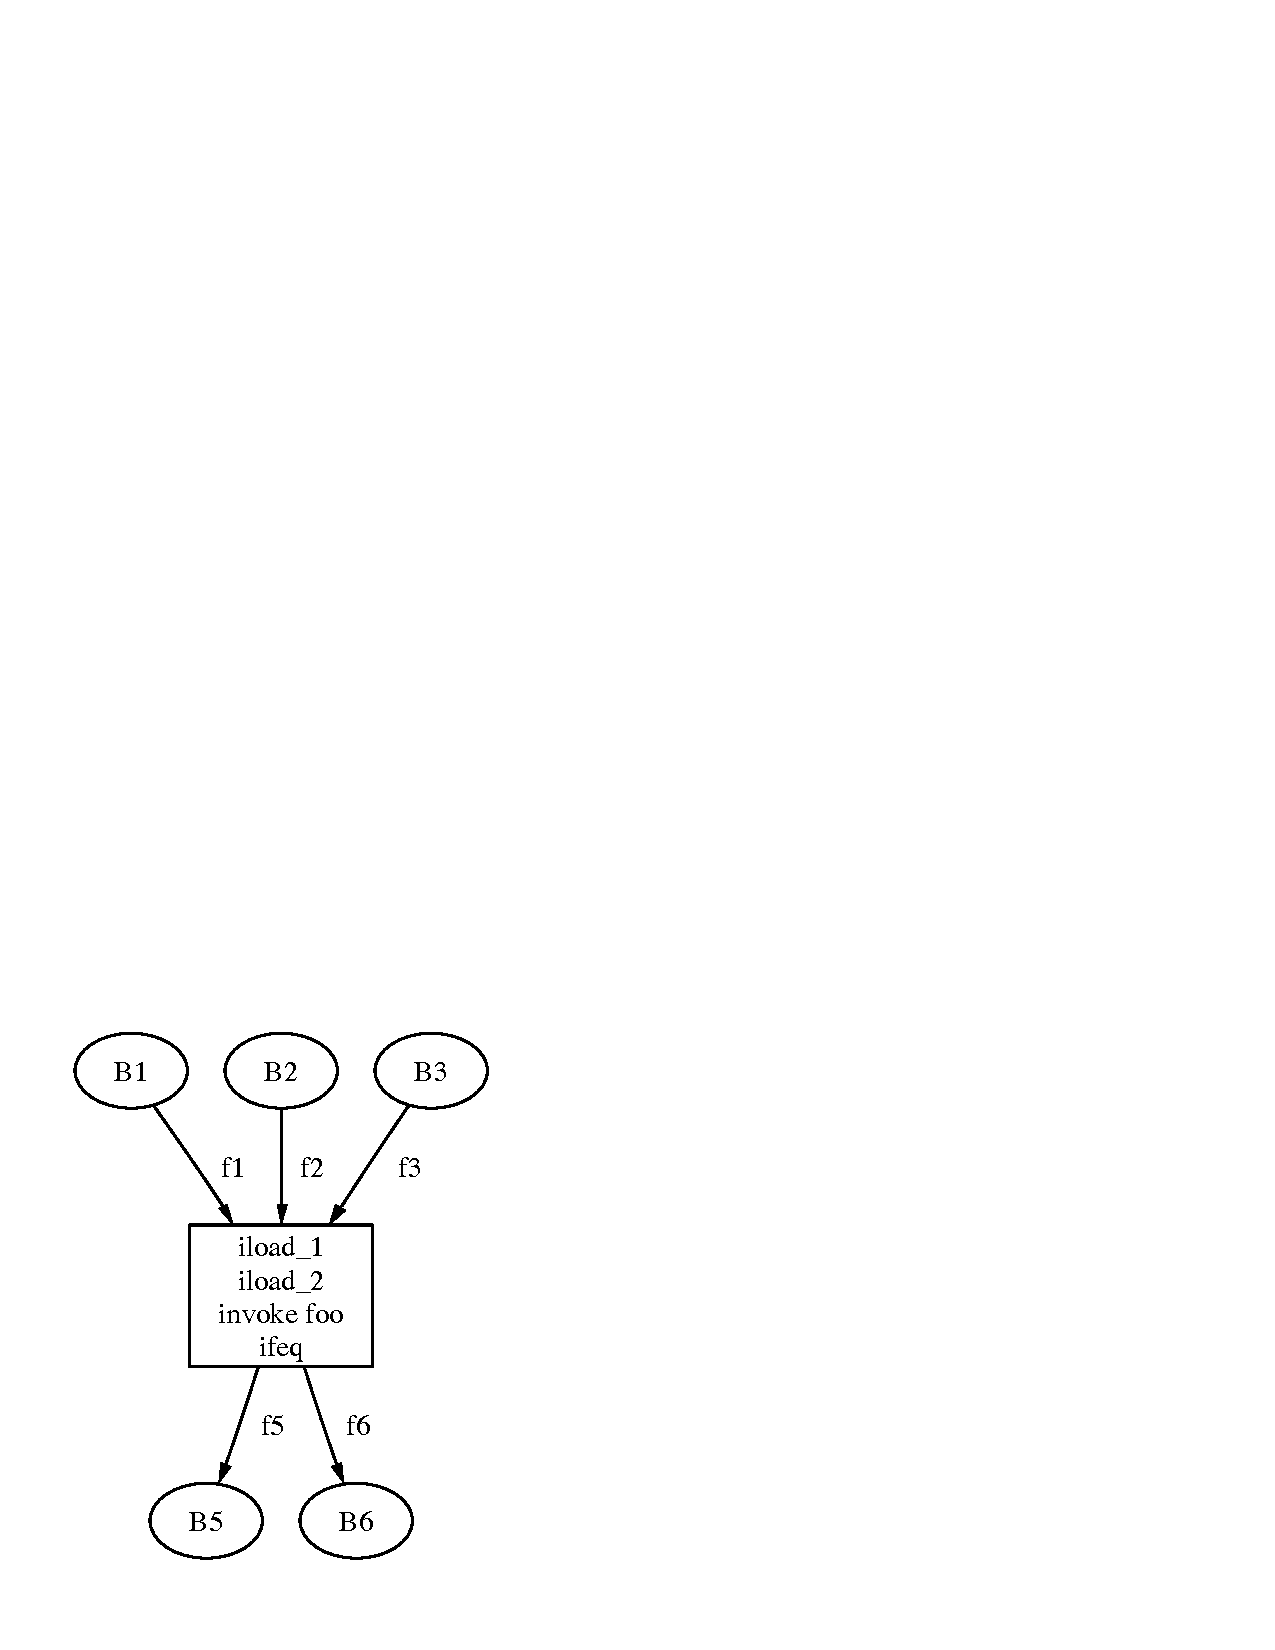
\includegraphics[scale=0.5]{wcet/cache_bb}
    \caption{Basic block with an invoke instruction}
    \label{fig:cache:bb}
\end{figure}

We split a basic block that contains a method invoke (B4 in our
example) into several blocks, so one block contains only the invoke
instruction. Misses on invoke and return are modeled as extra blocks
with the miss penalty as execution time.

The miss for the return happens during the return instruction. On a
miss, the caller method has to be loaded into the cache. Therefore,
the miss penalty depends on the caller method size. However, as the
return instruction is the last instruction executed in the called
method, we can model the return miss time at the caller side after
the invoke instruction. This approach simplifies the analysis as both
methods, the caller and the called, with their respective sizes, are
known at the occurrence of the invoke instruction.

Figure~\ref{fig:cache:split} shows the resulting graph after the
split of block B4 and the inserted vertices for the cache misses. The
miss penalty is handled in the same way as execution time of basic
blocks for the ILP objective function. The additional constraints for
the control flow in our example are
\begin{equation*}
    e_4 = f_{ih} + f_{im}
\end{equation*}
\begin{equation*}
    e_4 = f_{rh} + f_{rm}
\end{equation*}
with the invocation hit and miss frequencies $f_{ih}$ and $f_{im}$
and the return hit and miss frequencies $f_{rh}$ and $f_{rm}$.

\begin{figure}
    \centering
    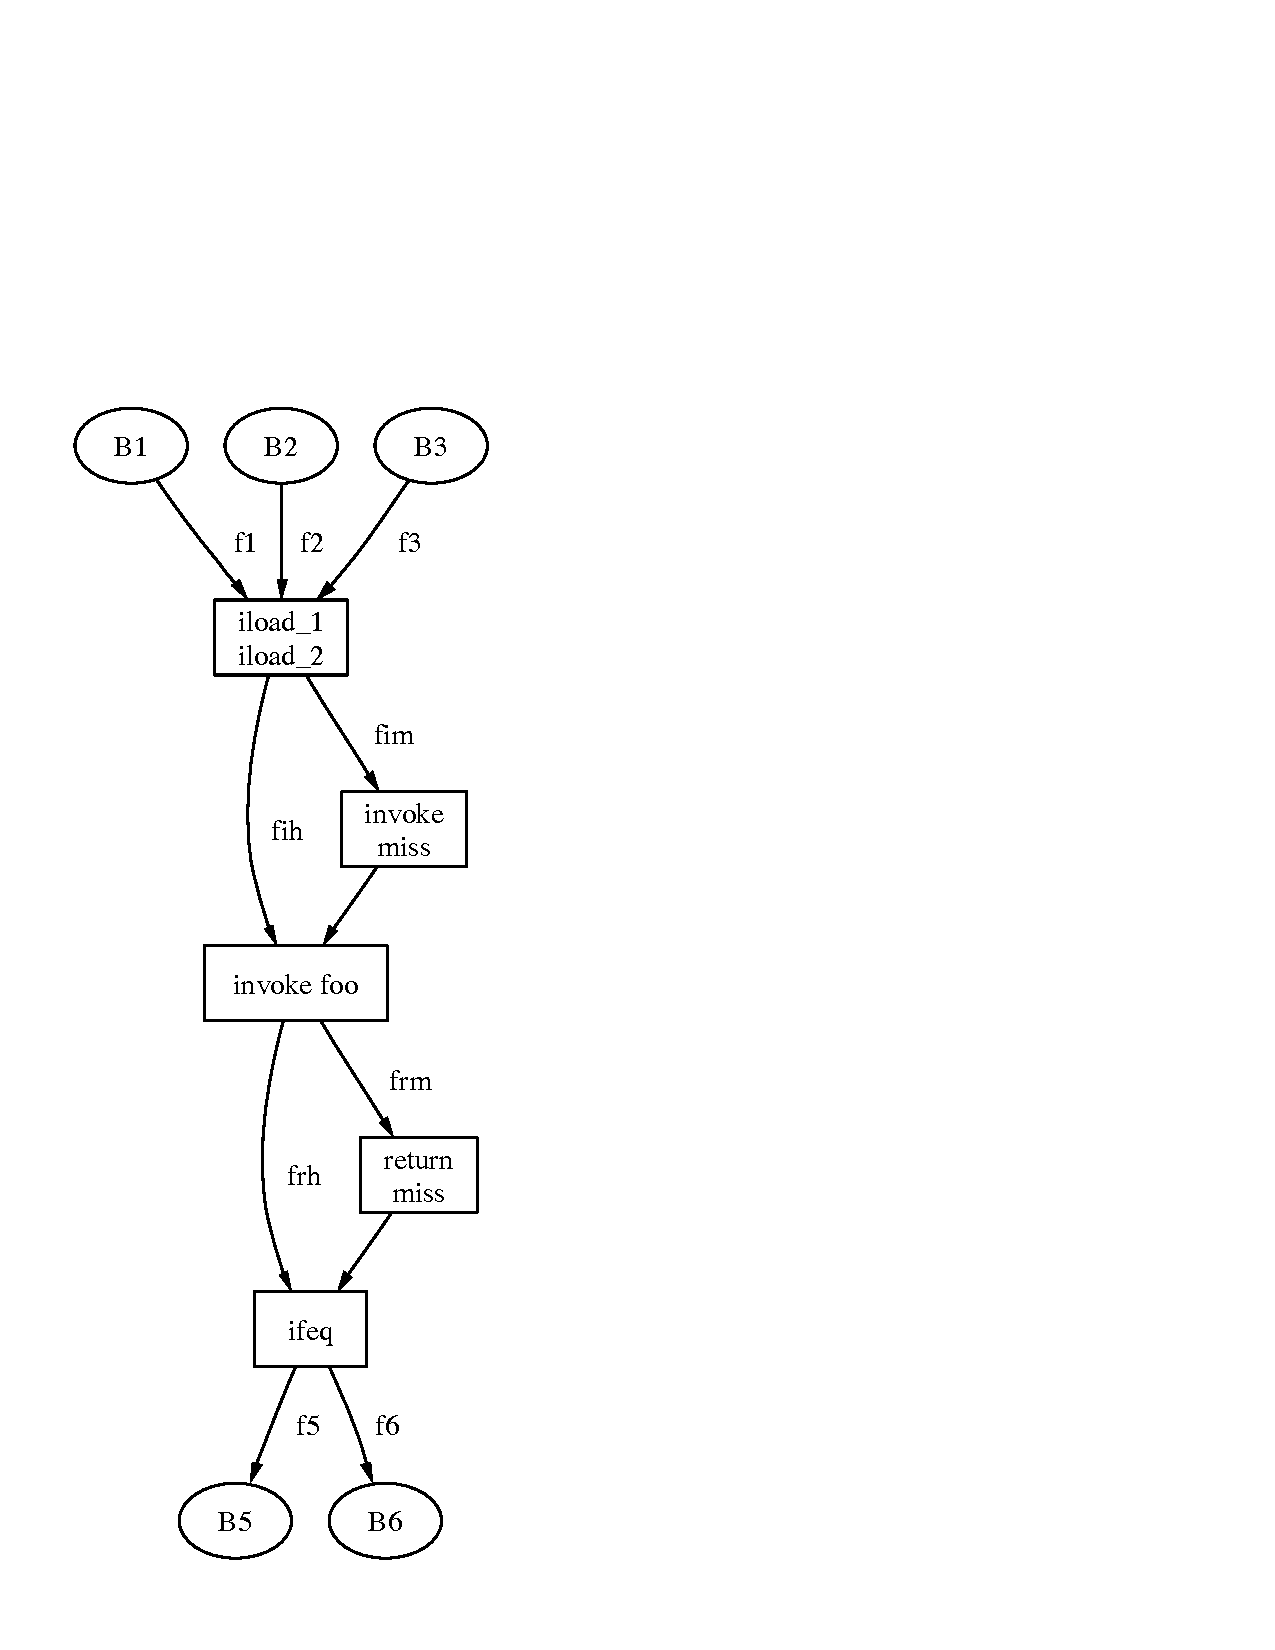
\includegraphics[scale=0.5]{wcet/cache_split}
    \caption{Split of the basic block and cache miss blocks}
    \label{fig:cache:split}
\end{figure}

It has to be noted that misses are always more expensive than hits. A
conservative bound on the hit frequency is a safe approximation when
the exact information is missing. As the hit or miss time is
contained within a single bytecode execution, there are no issues
with timing anomalies \cite{829103}.

\index{method cache!analysis}

As a next step, we have to formulate the relation between the hit and
the miss frequency. In \cite{jop:jtres_cache}, several variants of
the method cache are described:
\begin{enumerate}
    \item A single block that can only cache a single method
    \item Several blocks that each can cache a single method
    \item A variable block cache where a method can span several
        blocks
\end{enumerate}

The first two variants are simple to integrate into WCET analysis,
but lead to high WCET bounds. In the following, the analysis of the
third variant is described, details on analysis of the first two
variants can be found in \cite{jop:wcet:jtres06}.


%\subsection{Single Block Cache}
%
%The \emph{single block cache} can store only a single method.
%Therefore, it is very simple to analyze: Each invoke and each return
%results in a miss. We can include both miss times in the invoke
%execution time. It has to be noted that this single method cache
%still is a caching solution. The actual fetch of the bytecodes is
%from the cache. It provides a performance enhancement compared to a
%non-caching architecture.

% inner loops without invocations are also cached, e.g.

%\subsection{Dual Block Cache}
%\label{sec:two:block}
%
%A natural extension of the single block cache is the usage of
%several cache blocks, each one storing exactly one method. With more
%than one method in the cache, cache hit detection has to be performed
%as part of WCET analysis. Considering the minimal variant of two
%blocks, the analysis can be locally performed. We do not need to
%consider the whole program flow. We use a least recently used (LRU)
%replace strategy. LRU is quite natural for two blocks, as we fill the
%block that is not currently used.
%
%A cache hit on invoke or return can only happen when the invoked
%method is a leaf in the call tree. In that case, the cache contains
%the caller method and the called method. If we would invoke another
%method the former caller method would be replaced in the cache.
%
%As a conservative estimate, we only consider methods that are
%statically known to be leaves, i.e., methods that do not contain any
%invoke statement. Furthermore, we restrict the analysis to methods
%invoked within a loop. In that case the hit detection is as follows:
%\begin{description}
%    \item[Invoke] A hit on invoke is only possible if the method
%        is the same as the last invoked. That means a single
%        method invoked in a loop.\footnote{A second invocation of
%        the same method in straight line code, without an invoke
%        of a different method in between, will also result in a
%        hit.} In this case the first invocation is probably a
%        miss and all following invokes are guaranteed hits. With
%        the loop count $n$ and the execution frequency $f_h$
%        entering the loop head, the hit and miss frequencies are:
%\begin{eqnarray*}
%  f_{im} &=& f_h \\
%  f_{ih} &=& (n-1) f_h
%\end{eqnarray*}
%    \item[Return] A return is always a hit on the leaf as the caller
%    is still in the other block. In this case we can remove the miss
%    block from the graph.
%\end{description}
%
%Figure~\ref{fig:cache:loop} illustrates the invocation of a method in
%a loop. Basic block B2 is the loop head. With loop bound $n$, the
%resulting loop and cache constraints for this example are:
%\begin{eqnarray*}
%% \nonumber to remove numbering (before each equation)
%  f_2 &\le& n f_1\\
%  f_2 &=& f_{im} + f_{ih}\\
%  f_{im} &=& f_1 \\
%  f_{ih} &\le& (n-1) f_1
%\end{eqnarray*}
%
%\begin{figure}
%    \centering
%    \includegraphics[scale=0.5]{figures/cache_loop}
%    \caption{A method invocation in a loop}
%    \label{fig:cache:loop}
%\end{figure}
%
%It has to be noted that the cache constraints are conservative, as
%there could be another surrounding loop without a method invocation
%in the control flow.
%
%An extension of the two block cache to several blocks needs the
%whole control flow to model. Furthermore, reserving blocks for
%single methods is a waste of cache capacity. A better solution is
%described in the next section.


%\subsection{Variable Block Cache}
%% MS alternate text
%
%
% A practical approximation of the cache works as follows: Within a
% loop, all possibly invoked methods are tested if they will fit
% together into the cache. If this is the case, all methods miss at
% most once in the loop. However, the miss of a method that is not a
% leaf can happen on the return from an invoked method. As the miss
% penalty is different for an invoke bytecode and a return bytecode,
% this has to be taken into account. For JOP more cache load cycles can
% be hidden on an invoke. Therefore, the miss penalty on a return is
% higher. All methods from the fitting set that are not leaves need to
% consider one miss penalty of a return bytecode. Leaf nodes can
% naturally only miss on an invoke.

The \emph{variable block cache} divides the cache in several blocks
similar to cache lines in a conventional cache. However, a single
method has to be loaded in a continuous region of the cache. The
effective replacement policy of the variable block cache is FIFO.
FIFO caches need a long access history for standard classification
techniques \cite{Reineke:RTS2007}. Due to the FIFO replacement, one
can construct examples where a method in a loop can be classified as
single miss, but that miss does not need to happen at the first
iteration or it can happen on a return from an invoked method.



WCET analysis of cache hits for the method cache is most beneficial
for methods invoked in a loop, where the methods are classified as
first miss. The basic idea of the method cache analysis is as
follows: Within a loop it is statically analyzed if all methods
invoked and the invoking method, which contains the loop, fit
together in the method cache. If this is the case, all methods miss
at most once in the loop. The concrete implementation of the analysis
algorithm is a little bit different.

However, the miss of a method that is not a leaf method can happen
either at invoke of this method or on the return (from a deeper
nested method) to this method. On JOP some of the cache load cycles
can be hidden due to the concurrent execution of microcode. At the
more complex invoke instruction more cash load time is hidden.
Therefore, the miss penalty on a return is higher. All methods from
the fitting set that are not leafs need to consider the miss penalty
of a return bytecode. Leaf nodes can naturally only miss on an
invoke.

With the variable block cache, it could be argued that WCET analysis
becomes too complex, but the technique presented above is easy to
apply and only needs to perform a simple static analysis. In contrast
to a direct-mapped instruction cache, we only need to consider invoke
instructions and do not need to know the actual bytecode address of
any instruction.


%% text from BH
%
%Therefore, instead of classifying one particular cache access, we
%bound the number of cache misses during the execution of a method or
%loop. This approach, is based on the following fact for $N$ block
%FIFO caches: If it is known that during the execution of a code
%region, at most $N$ distinct cache blocks are accessed, each accessed
%block will be loaded \emph{at most once}. For example, suppose all
%methods invoked during the execution of a loop, together with the
%method containing the loop, fit into the cache. Then for every method
%possibly accessed during the execution, at most one cache access will
%be a cache miss.
%
%The quality of this approximation depends on the heuristic used to
%check whether at most $N$ distinct cache blocks are accessed. We
%found that simply considering all methods possibly invoked works well
%enough, but better results may be obtained using a more sophisticated
%check.
%
%Furthermore, this approximation requires call context dependent
%constraints, i.e., the constraint that at most one cache access is a
%miss only applies to those cache access during the execution of the
%code region. As context dependencies cannot be directly expressed
%using linear constraints, we duplicate the affected CFGs in the ILP
%model.
%
%% ILP integration
%To include the cache analysis in the ILP model, we traverse the
%callgraph of the program starting from the root method. We check for
%each call site, whether no more than $N$ cache blocks are loaded
%during the execution of the invoked method. If this is the case, the
%subgraph rooted at the invoked method is duplicated. For each method
%in that graph, we add the constraint that at most one of the cache
%accesses to the method is a miss.

%
%An example, shown in Listing~\ref{lst:varcacheJava}, demonstrates the
%idea of the cache analysis. Assume that methods $a$, $b$ and $c$
%together fit into the cache, but not $a$, $b$, $c$ and $m$. The cache
%miss frequency variables for the methods in the example are given in
%the comment, e.g., $f_1$ for a miss on invoking method $a$ and $f_2$
%for a miss when method $a$ returns.
%\begin{lstlisting}[float, caption={FIFO Cache Analysis},label=lst:varcacheJava]
%
%  m() {
%      a();  /* f1 (invoke a), f2 (return to m) */
%  }
%  a() {
%      b();  /* f3 (invoke b), f4 (return to a) */
%      c();  /* f5 (invoke c), f6 (return to a) */
%  }
%  b() {
%      c();  /* f7 (invoke c), f8 (return to b) */
%  }
%  c() {
%  }
%\end{lstlisting}
%During the execution of $a$, as all three methods fit into the cache,
%each of the methods $a$, $b$ and $c$ will be missed at most once.
%Therefore, we add the constraints
%\begin{eqnarray*}
%   f_1 + f_4 + f_6 &\leq& 1 \\
%   f_3 + f_8          &\leq& 1 \\
%   f_5 + f_7          &\leq& 1
%\end{eqnarray*}
%Due to this constraints, either $f_5$ or $f_7$ is executed once on
%the worst case path, but not both of them. On JOP, return
%instructions are always more expensive than invoke instructions, and
%so $f_8 = 1$ and $f_3 = 0$. For $a$, $f_1 = 0$ and either $f_4 = 1$
%or $f_6 = 1$. If $a$ is also invoked from some other call site, we
%need to duplicate the timing graph for $a$, $b$ and $c$.


%% MS: ref CP for CMP extension and add tool + argue about 15%+
%% with new tool for CMP due to better cache analysis and more
%% preassure on memory bandwidth




\subsection{WCET Analyzer}
\index{WCET!tool}

The WCET analyzer (WCA) is an open source Java program first
described in \cite{jop:wcet:jtres06} and later redesigned
\cite{master:huber:2009}. It is based on the standard IPET approach
\cite{Puschner:JRTS1997}, as described in Section~\ref{sec:ilp}.
Hereby, WCET is computed by solving a maximum cost circulation
problem in a directed graph representing the program's control flow.
In contrast to the former description, WCA associates the execution
cost to the edges instead of the vertices. For modeling the execution
time of JOP those two approaches are equivalent. However, WCA is
prepared for other architectures with different execution times of a
branch taken or not taken.

The tool performs the low-level analysis at the bytecode level. The
behavior of the method cache is integrated with the static all-fit
approximation (see Section~\ref{sec:wcet:cache}). The well known
execution times of the different bytecodes (see
Section~\ref{sec:wcet:bc}) simplify this part of the WCET analysis,
which is usually the most complex one, to a great extent. As there
are no pipeline dependencies, the calculation of the execution time
for a basic block is merely just adding the individual cycles for
each instruction.

To access the class files, we use the Byte Code Engineering Library
(BCEL) \cite{gc:bcel}. BCEL allows inspection and manipulation of
class files and the bytecodes of the methods. The WCA extracts the
basic blocks from the methods and builds the CFG. Within the CFG, the
WCA detects both the loops and the loop head. From the source line
attribute of the loop head, the annotation of the loop count is
extracted. WCA uses the open-source ILP solver \code{lp\_solve}.
\code{lp\_solve} is integrated into the WCA by directly invoking it
via the Java library binding.

After completing WCET analysis, WCA creates detailed reports to
provide feedback to the user and annotate the source code as far as
possible. All reports are formatted as HTML pages. Each individual
method is listed with basic blocks and execution time of bytecodes,
basic blocks, and cache miss times. This output is similar to
Table~\ref{tab:wcet:bytecode}, but with more detailed information.
The WCA also generates a graphical representation of the CFG for each
method and for the whole program. Furthermore, the source is
annotated with execution time and the WCET path is marked, as shown
in Figure~\ref{fig:report} for the example from
Listing~\ref{lst:wcet:example}. For this purpose, the solution of the
ILP is analyzed, first annotating the nodes of the CFG with execution
costs, and then mapping the costs back to the source code.


\begin{figure}[t]
  \centering
  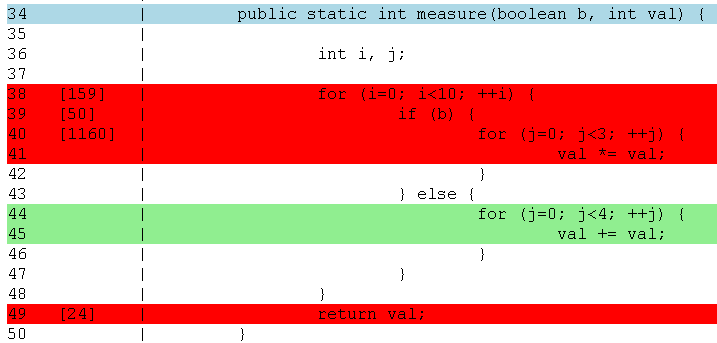
\includegraphics[scale=0.5]{wcet/html}\\
  \caption{WCET path highlighting in the source code.}\label{fig:report}
\end{figure}

The \code{Makefile} contains the target \code{wcet} for the WCET
tool. The following example performs WCET analysis of the method
\code{measure} of the \code{crc} example and uses DFA for the loop
bound detection. The method that is the root of the application to be
analyzed can be set in variable \code{WCET\_METHOD}.
\begin{lstlisting}
    make java_app wcet -e P1=test P2=wcet P3=ShortCrc WCET_DFA=yes
\end{lstlisting}

\section{Evaluation}
\label{sec:wcet:eval}

For the evaluation of the WCET tool, we analyze and measure a
collection of real-time benchmarks. The measurement gives us
confidence that we have no serious bugs in the analysis and an idea
of the pessimism of the analyzed WCET. It has to be noted that we
actually cannot guarantee to measure the real WCET. If we could
measure the WCET, we would not need to perform WCET analysis at all.

Furthermore, WCET analysis gives a safe bound, but this bound may be
conservative. Due to the abstractions in the analysis the WCET bound
may not be associated with a real feasible execution path. There is
no general guarantee that we have knowledge about the worst case
path.


\subsection{Benchmarks}
\label{sec:benchmarks}

\begin{table}[t]
\begin{center}
\begin{small}
\begin{tabular}{lllr}
    \toprule
    Benchmark   & Program             & Description                         & LOC \\
    \midrule
    Kernel      & crc          & CRC calculation for short messages  & 8 \\
                & LineFollower & A simple line follower robot        & 89 \\
                & SVM          & Embedded machine learning algorithm & 115 \\
    \midrule
    M\"alardalen & BinarySearch&  Binary search program              & 78 \\
                & Bubble       &  Bubblesort program                 & 63 \\
                & Crc          &  Cyclic redundancy check            & 154 \\
                & ExpInt       &  Exponential integral function      & 89 \\
                & FDCT         &  Fast discrete cosine transform     & 222 \\
                & Fibonacci    &  Simple iterative Fibonacci calculation & 37 \\
                & InsertionSort&  Insertion sort program             & 60 \\
                & JanneComplex &  Complex nested loops               & 72 \\
                & MatrixCount  &  Count numbers in a matrix          & 85 \\
                & MatrixMult   &  Matrix multiplication              & 104 \\
                & NestedSearch &  Search in a multi-dimensional array& 487 \\
%    PetriNet     &  Petri Net simulation                 & 4008 \\
                & QuickSort    &  Quicksort program                  & 166  \\
                & Select       &  Select smallest element from array & 136  \\
                & SLE          &  Simultaneous linear equations      & 128  \\
    \midrule
    Applications& Lift         & Lift controller                     & 635 \\
                & Kfl          & \emph{Kippfahrleitung} application  & 1366 \\
%    UdpIp & UDP/IP benchmark & 1297 \\
                & EjipCmp      & Multicore UDP/IP benchmark          & 1892 \\
    \bottomrule
\end{tabular}
\end{small}
\end{center}
    \caption{WCET benchmark examples}
    \label{tab:wcet:examples}
\end{table}


The benchmarks used are shown in Table~\ref{tab:wcet:examples}, with
a short description and the source code size in lines of code (LOC).
The benchmarks consists of three groups: small kernel benchmarks,
WCET benchmarks provided by the M\"alardalen Real-Time Research
Center,
 \footnote{Freely available from \url{http://www.mrtc.mdh.se/projects/wcet/benchmarks.html}}
and three real-world applications.

The benchmark \code{crc} calculates a 16-bit CRC for short messages.
\code{LineFollower} is the code of a simple line-following robot. The
\code{SVM} benchmark represents an embedded version of the machine
learning algorithm called support vector machine (SVM). The SVM is
modified minimally to work in the real-time setting
\cite{hardreal2006pedersen}. The second group are benchmarks provided
by the M\"alardalen Real-Time Research Center \cite{mrtc:bench} and
ported to Java by Trevor Harmon \cite{jop:volta:rtas2008}.

The benchmarks \code{Lift} and \code{Kfl} are real-world examples
that are in industrial use. \code{Lift} is a simple lift controller,
where \code{Kfl} is a node in a distributed mast control application.
The \code{EjipCmp} benchmark is an embedded TCP/IP stack written in
Java with an example application consisting of a UDP/IP server and a
UDP/IP client, exchanging messages via a loopback network layer
driver. The TCP/IP stack and the example applications are optimized
for a chip-multiprocessor system (e.g., with non-blocking
communication). In our setup, however, we execute all five tasks
serially on a uniprocessor and perform WCET analysis for the
aggregation of the five tasks.


The configuration of JOP for the evaluation is with a 4~KB method
cache configured for 16 blocks. The memory access times are 2 cycles
for a read and 3 cycles for a write.


\subsection{Analysis and Measurements}
\label{sec:benchwcet}

%% MS: notes on the Ejip benchmark
%% Tftp (in Udp.java) and Html (in Net.java) disabled for Net.run() analysis.
%% Also changes in the IP checksum calculation
%% TODO if EjipCmp is further used as WCET example
%%  1. find out why new checksum does not work
%%  2. make TFTP and HTML handler optional
%%      -> change OEBB, TAL, and example applications

\begin{table}[t]
\begin{center}
\begin{small}
\begin{tabular}{lrrr}
    \toprule
%    & \multicolumn{3}{c}{WCET}  \\
%    \cmidrule(lr){2-4}
     & Measured & Estimated & Pessimism \\
    Program             & (cycles) & (cycles) & (ratio) \\
    \midrule
    crc          &     1449 &   1513 & 1.04 \\ %  -- old WCA value was 1513?
    LineFollower &     2348&    2411 & 1.03 \\ %  -- old WCA 2589, now 2451 with WCA
    SVM          &  104880 &  107009 & 1.02 \\
    \midrule
    BinarySearch &     631 &     636 & 1.01  \\
    % Return miss cost additional 5 cycles (min-cache-cost is 631)
    Bubble       & 1262717 & 1815734 & 1.44 \\
    Crc          &  191825 &  383026 & 2.00 \\
    ExpInt       &  324419 &  429954 & 1.33 \\
    FDCT         &   19124 &   19131 & 1.00 \\
    Fibonacci    &    1127 &    1138 & 1.01 \\
    InsertionSort&    8927 &   15410 & 1.73 \\
    JanneComplex &     886 &    6991 & 7.89 \\
    MatrixCount  &   16420 &   16423 & 1.00 \\
    MatrixMult   & 1088497 &  1088509& 1.00 \\
    NestedSearch &   51777 &   64687 & 1.25 \\
%    PetriNet    &  & 1/1 \\ too large
    QuickSort    &    9942 &  115383 & 11.61 \\
    Select       &    5362 &   55894 & 10.42 \\
    SLE          &   20408 &   50514 & 2.48 \\
    \midrule
    Lift         &    5446 &    8466 & 1.55 \\
    Kfl          &   10411 &   39555 & 3.80 \\
% Kfl without service path:  22875  2.20
%    UdpIp       &       8316 &  182569 & 21.95&   10   &  78  &  6/12\\
    EjipCmp      &   15297 &   21965 & 1.44 \\
    \bottomrule
\end{tabular}
\end{small}
\end{center}
    \caption{Measured and estimated WCET with result in clock
    cycles}
    \label{tab:wcet:compared}
\end{table}

%% MS: on Kfl pessimism:
%% an infisible path annotation at
%				if (state == BBSys.MS_SERVICE) {
%					doService();		// never return!
%				}
%% would result in a pessimism of 2.5

%\emph{TODO: on programming style of KFL: The dispatch of commands is
%done in several if statements where in fact only one statement can be
%true. However, this fact is not considered in the WCet analysis. Bad
%style for WCET - a switch statement of if else chain would be better.
%Not really as each if contains a return.}
%
%\emph{TODO: write on cache miss for the return to the measure()
%method. Define what we mean when doing WCET analysis of method
%m(): no invoke m() included, no cache miss on invoke m() included,
%but the cache miss for a return to m() is included although it is not
%part of the measurement. Perhaps show the code snipped that is used
%to measure a method.}

Table~\ref{tab:wcet:compared} shows the measured execution time and
the analyzed WCET. The last column gives an idea of the pessimism of
the WCET analysis. It has to be noted (again) that we actually cannot
guarantee to measure the real WCET. If we could measure the WCET, we
would not need to perform WCET analysis at all. The WCET analysis
result of a method is defined as follows: WCA reports the WCET of the
executable code within a method including the return statement. The
invoke of the to-be-analyzed method is not part of the analysis. With
respect to cache analysis the return from the method does not include
any miss time -- invoke and return miss time are considered as part
of the invoke instruction. For the measurement we use a cycle counter
and take a time stamp before the first instruction of the method and
after the return from the method.

For very simple programs, such as \code{crc}, \code{robot}, and
\code{SVM} the pessimism is quite low. The same is true for several
of the benchmarks from the M\"alardalen benchmark suit. Some are
almost cycle accurate. The small overestimation of, e.g., 5 cycles
for \code{BinarySearch}, results from our measurement methodology and
the definition of what the WCET of a single method is. To avoid
instrumenting all benchmarks with time stamp code we wrap the
benchmarks in a method \code{measure()}, vary which benchmark is
invoked in \code{measure()}, and analyze this method. Therefore,
\code{measure()} contains an invoke and the control is return to
\code{measure()}. In the case of small benchmarks the method cache
still contains \code{measure()} on the return from the benchmark
method. However, WCA does not include \code{measure()} as a possible
method for the static method cache analysis (it is performed on a
invoke and no invoke of \code{measure()} is seen by WCA). Therefore,
the return from the benchmark method is classified as miss.

The pessimism of most of the other benchmarks, including the two
applications \code{Lift} and \code{EjipCmp}, are in an acceptable
range below a factor of 2. Three benchmarks, \code{JanneComplex},
\code{QuickSort}, and \code{Select}, stand out with a high pessimism.
\code{JanneComplex} is an artificial benchmark with a complex loop
dependency of an inner loop and the annotation results in a
conservative estimation. However, it has to be noted that the
benchmarks from M\"alardalen are designed to challenge WCET tools. We
assume that a safety-critical programmer would not use
\code{QuickSort} as a first choice for time-predictable code.

%\code{InsertionSort} is a challenge for WCET tools as it contains a
%triangular loop with data dependent loop execution of the inner loop.

The pessimism of \code{Kfl} is quite high. The difference between the
measurement, and the analysis in the \code{Kfl} example, results from
the fact that our measurement does not cover the WCET path. We only
simulate input values and commands for the mission phase. However,
the main loop of \code{Kfl} also handles service functions. Those
functions are not part of the mission phase, but make up the WCET
path. If we omit the non-feasible path to the service routine the
WCET drops down to 22875 and the overestimation is 2.2.

% Kfl without service path:  22875  2.20


%The large conservatism in \code{UdpIp} results from the loop bound in
%the IP and UDP checksum calculation. It is set for a 1500 byte packet
%buffer that can be handled by our UDP/IP stack. However, in the
%benchmark the UDP payload is only 8 bytes. When setting this loop
%bound according to the benchmark, the WCET drops to 12515 cycles.

%% MS: The UdpIp benchmark uses now shorter package buffers, but
%% is annotated for the 1500 byte buffer. The numbers are therefore
%% *without* DFA.

The \code{Kfl} example show the issue when a real-time application is
developed without a WCET analysis tool available. Getting the
feedback from the analysis earlier in the design phase can help the
programmer to adapt to a WCET aware programming style. In one
extreme, this can end up in the single-path programming style
\cite{pusch02:single:path}. A less radical approach can use some
heuristics for a WCET aware programming style. For instance, avoiding
the service routines in the application main loop.

%E.g.\ for the \code{UdpIp} example a \emph{special} version of the
%UDP and IP checksum calculation for short messages can be added to
%the UDP/IP stack.

The results given in Table~\ref{tab:wcet:compared} are comparable to
the results presented in \cite{jop:wcet:jtres06}. Most benchmarks now
take less cycles than in 2006 as the performance of JOP has been
advanced. The exceptions are two benchmarks, \code{LineFollower} and
\code{Kfl}, which now have a higher WCET. The line-following robot
example was rewritten in a more object-oriented way. Finally, the
different number for the \code{Kfl} resulted from a bug in the WCA
that was corrected after the publication in 2006.

\section{Discussion}
\label{sec:wcet:discussion}

We found that the approach of a time-predictable processor and static
WCET analysis is a feasible solution for future safety-critical
systems. However, there are some remaining questions that are
discussed in the following sections.

\subsection{On Correctness of WCET Analysis}

Safe WCET approximation depends on the correct modeling of the target
architecture and the correct implementation of the analysis tools.
During the course of this paper we have found a bug in the WCA from
2006 and have also found bugs in the low-level timing description of
JOP. However, the open-source approach for the processor and the
tools increases the chance that bugs are found. Furthermore, we have
compared the results of the new implementation of WCA with two
independent implementations of WCET analysis for JOP: The Volta
project by Trevor Harmon \cite{Trevor:Volta} and the former
implementation of WCA \cite{jop:wcet:jtres06}. The results differ
only slightly due to different versions of JOP that Volta, used and a
less accurate cache analysis implemented in the second tool. It
should be noted that JOP and the WCA are still considered on-going
research prototypes for real-time systems. We would not (yet) suggest
to deploy JOP in the next safety-critical application.

\subsection{Is JOP the Only Target Architecture?}

JOP is the primary low-level target for the WCET analysis tool as it
is: (a) a simple processor, (b) open-source, and (c) the execution
timing is well-documented (see Appendix~\ref{appx:bytecode}).
Furthermore, the JOP design is actually the root of a family of Java
processors. Flavius Gruian has built a JOP compatible processor, with
a different pipeline organization, with Bluespec Verilog
\cite{flavius:bluejep}. The SHAP Java processor \cite{shap}, although
now with a different pipeline structure and hardware assisted garbage
collection, also has its roots in the JOP design. We assume that
these processors are also WCET analysis \emph{friendly}. The question
remains how easy the analysis can be adapted for other Java
processors.


The same analysis is not possible for other Java processors. Either
the information on the bytecode execution time is missing\footnote{We
tried hard to get this information for the aJile processor.} or some
processor features (e.g., the high variability of the latency for a
trap in picoJava) would result in very conservative WCET estimates.
Another example that prohibits exact analysis is the mechanism to
automatically fill and spill the stack cache in picoJava
\cite{pjMicroArch,pjProgRef}. The time when the memory (cache) is
occupied by this spill/fill action depends on a long instruction
history. Also the fill level of the 16-byte-deep prefetch buffer,
which is needed for instruction folding, depends on the execution
history. All these automatic buffering features have to be modeled
quite conservatively. A pragmatic solution is to assume empty buffers
at the start of a basic block. As basic blocks are quite short, most
of the buffering/prefetching does not help to lower the WCET.

Only for the Cjip processor is the execution time well documented
\cite{CjipRef}. However, the \emph{measured} execution time of some
bytecodes is \emph{higher} than the documented values
\cite{jop:thesis}. Therefore the documentation is not complete to
provide a safe processor model of the Cjip for WCET analysis.

The real-time Java processor jamuth \cite{jamuth:jtres07} is a
possible target for the WCA. There is on-going work with Sascha Uhrig
to integrate the timing model of jamuth into the WCA. A preliminary
version of that model has been tested. The analysis tool need to be
changed to model a few pipeline dependencies.

Still, WCET analysis of Java programs on RISC processors with a
compiling JVM is a challenge. With a compiling JVM, the WCET friendly
bytecodes are further compiled into machine code. Information is lost
in the second transformation. This is not the case with a dedicated
Java processor such as JOP.

\subsection{Object-oriented Evaluation Examples}

Most of the benchmarks used are written in a rather conservative
programming style. The M\"alardalen benchmarks are small kernels that
do not stress the cache analysis. We would like to use more
object-oriented real-time examples for the evaluation. Then, we can
evaluate if object-oriented programming style with dynamic method
dispatch and rather small methods is a feasible option for future
real-time systems.

\subsection{WCET Analysis for Chip-multiprocessors}

Chip-multiprocessors (CMP) are now considered as the future
technology for high-performance embedded systems. Christof Pitter has
built a CMP version of JOP that includes a time-predictable memory
arbiter \cite{phd:pitter}. During the course of his thesis he has
adapted the low-level timing calculation of the WCET tool to
integrate the memory access times with the time-sliced arbiter.
Therefore, it is possible to derive WCET values for tasks running on
a CMP system with shared main memory. To best of our knowledge, this
is the first time-predictable CMP system where WCET analysis is
available.

The first estimation of bytecode timings for the CMP system considers
only individual bytecodes. However, with variable memory access times
due to memory arbitration this estimate is conservative. An extension
to basic block analysis and using model checking to analyze possible
interactions between the memory arbitration process and the program
execution should result in tighter WCET estimates.

The JOP CMP system showed the importance of tighter method cache
analysis. Compared to the simple approach of the original WCA tool,
the new static cache approximation yielded in 15\% tighter WCET
estimates for a 8 core CMP system.

%% not yet to publish
%\subsubsection{Data Cache}
%
%In JOP only the stack content is stored in fast on-chip memory.
%Access to object and array fields goes directly to main memory. This
%setup is good enough for a uniprocessor solution with fast main
%memory (e.g., SRAM). However, for a CMP version of JOP the memory
%bandwidth becomes the bottleneck and we have added a data cache with
%high associativity and least-recently used (LRU) replacement policy
%to JOP. The high associativity is intended to allow WCET analysis of
%heap accesses where the addresses are not statically known.
%
%As a first approach, we will include data cache analysis similar to
%the method cache analysis. Within loops the number of heap accesses
%to different addresses (different references plus field/array
%offsets) is determined. If that number is lower than the
%associativity we can qualify all heap accesses as a single miss for
%one loop iteration and hits for the other iterations. With this type
%of analysis two replacement policies are feasible: LRU and FIFO. FIFO
%consumes a little bit less resources than LRU, but the main issue,
%with respect to resources and hit detection time, is the high
%associativity.

\subsection{Co-Development of Processor Architecture and WCET
Analysis}

JOP is an example of a time-predictable computer architecture. An
extension of this approach to RISC and VLIW based processors is
presented in \cite{tpca:jes}. We consider a co-development of
time-predictable computer architecture and WCET analysis for the
architectural features as an ideal approach for future real-time
systems. A new time-predictable feature (e.g., a data cache
organization) can only be evaluated when the analysis is available.
The analysis, and what can be analyzed within practical execution
time and memory demands, shall guide the computer architect of future
time-predictable processors.

\subsection{Further Paths to Explore}

The combination of a bytecode based optimizer (a prototype is
available as part of the JOP sources) with WCET analysis can be
applied to minimize the WCET path. The optimizer can be guided by the
results from the application. This iterative flow can be used to
minimize the worst-case path instead of the average-case path in the
application.

%
%\begin{itemize}
%  \item DFA extension for triangular loops
%  \item Call string in WCET
%  \item Model checking for cache analysis
%\end{itemize}
%

%\subsubsection{WCET Optimized Programming}
%
%\begin{itemize}
%  \item Optimize the 'real' WCET
%  \item Help the DFA -- DFA friendly programming
%\end{itemize}



\section{Summary}
\label{sec:wcet:summary}

In this chapter, the WCET analysis tool based on the ILP approach has
been presented. The architecture of the Java processor greatly
simplifies the low-level part of WCET analysis, as it can be
performed at the Java bytecode level. An instruction cache, named
\emph{method cache}, stores complete methods, and is integrated into
the WCET analysis tool.

The WCET analysis tool, with the help of DFA detected loop bounds,
provides WCET values for the schedulability analysis. Complex loops
still need to be annotated in the source. A receiver type analysis
helps to tighten the WCET of object-oriented programs. We have also
integrated the method cache into the analysis. The cache can be
analyzed at the method level and does not need the full program CFG.
Besides the calculation of the WCET, the tool provides user feedback
by generating bytecode listings with timing information and a
graphical representation of the CFG with timing and frequency
information. This representation of the WCET path through the code
can guide the developer to write WCET aware real-time code.

The experiments with the WCET analyzer tool have demonstrated that we
have achieved our goal: JOP is a simple target for WCET analysis.
Most bytecodes have a single execution time (WCET = BCET), and the
WCET of a task (the analysis at the bytecode level) depends only on
the control flow. No pipeline or data dependencies complicate the
low-level part of WCET analysis.

\section{Further Reading}
\label{sec:wcet:related}

There are a lot of papers available on WCET analysis and modeling of
low-level processor features. This section gives an overview of the
related work for our WCET analyzer.

\subsection{WCET Analysis}

Shaw presents in \cite{Shaw:timeschema} timing schemas to calculate
minimum and maximum execution time for common language constructs.
The rules allow to collapse the CFG of a program until a final single
value represents the WCET. However, with this approach it is not
straight forward to incorporate global low-level attributes, such as
pipelines or caches. The resulting bounds are not tight enough to be
practically useful.

Computing the WCET with an integer linear programming (ILP) solver is
proposed in \cite{Puschner:JRTS1997} and \cite{216666}. The approach
is named graph-based and implicit path enumeration respectively. We
base our WCET analyzer on the ideas from these two groups.

The WCET is calculated by transforming the calculation to an integer
linear programming problem. Each basic block\footnote{A basic block
is a sequence of instructions without any jumps or jump targets
within this sequence.} is represented by an edge $e_i$ in the T-graph
(timing graph) with the weight of the execution time of the basic
block. Vertices $v_i$ in the graph represent the split and join
points in the control flow. Furthermore, each edge is also assigned
an execution frequency $f_i$. The constraints resulting from the
T-graph and additional functional constraints (e.g.\ loop bounds) are
solved by an ILP solver. The T-graph is similar to a CFG, where the
execution time is modeled in the vertices. The motivation to model
the execution time in the edges results from the observation that
most basic blocks end with a conditional branch. A conditional branch
usually has a different execution time, depending on whether it is
taken or not. This difference is represented by two edges with
different weights.

In \cite{216666} a similar approach with ILP is proposed. However,
they use the CFG as the basis to build the ILP problem. The approach
is extended to model the instruction cache with cache conflict
graphs. The evaluation with an Intel i960 processor shows tight
results for small programs \cite{828940}. However, the conservative
modeling of the register window (overflow/underflow on each function
call/return) adds 50 cycles to each call and return. This observation
is another argument for a WCET aware processor architecture.

WCET analysis of object-oriented languages is presented by Gustafsson
\cite{gustafsson:phd}. Gustafsson uses abstract interpretation for
automatic flow analysis to find loop bounds and in feasible paths.
The work is extended to a modular WCET tool with instruction cache
analysis and pipeline analysis \cite{eng:jnl:2003}.
%% MS: shall we keep the following paper? It is a little bit weak.
A summary of new complexities to WCET analysis is given in
\cite{gustafsson:words:2002}.


Cache memories for the instructions and data are classic examples of
the paradigm: \emph{Make the common case fast}. Avoiding or ignoring
this feature in real-time systems, due to its unpredictable behavior,
results in a very pessimistic WCET bound. Plenty of effort has gone
into research to integrate the instruction cache into the timing
analysis of tasks \cite{Arnold1994,Healy1995}, the cache's influence
on task preemption \cite{279589,Mataix:1996}, and integration of the
cache analysis with the pipeline analysis \cite{wcet:healy:1999}.
Heckmann et.\ al described the influence of different cache
architectures on WCET analysis \cite{Heckmann:IEEE2003}.

An overview of WCET related research is presented in
\cite{R:Puschner:2000} and \cite{tecs:wcet:overview}.



\subsection{WCET Analysis for Java}

WCET analysis at the bytecode level became a research topic, at the
time Java was considered for future real-time systems. WCET analysis
at the bytecode level was first considered in \cite{R:Bernat:2000a}.
It is argued that the well formed intermediate representation of a
program in Java bytecode, which can also be generated from compilers
for other languages (e.g.\ Ada), is well suited for a portable WCET
analysis tool. In that paper, annotations for Java and Ada are
presented to guide WCET analysis at bytecode level. The work is
extended to address the machine-dependent low-level timing analysis
\cite{R:Bate:2000a}. Worst-case execution frequencies of Java
bytecodes are introduced for a machine independent timing
information. Pipeline effects (on the target machine) across bytecode
boundaries are modeled by a \emph{gain time} for bytecode pairs.

In \cite{871917} a portable WCET analysis is proposed. The abstract
WCET analysis is performed on the development site and generates
abstract WCET information.
%
%Scopes and markers \cite{84850} are used to get a tighter bound of
%the WCET.
%
The concrete WCET analysis is performed on the target machine by
replacing abstract values within the WCET formulae by the machine
dependent concrete values.

In \cite{R:Bate:2002c}, an extension of \cite{R:Bernat:2000a} and
\cite{R:Bate:2000a}, an approach how the portable WCET information
can be embedded in the Java class file is given. It is suggested that
the final WCET calculation is performed by the target JVM. The
calculation is performed for each method and the static call tree is
traversed by a recursive call of the WCET analyzer.


\subsection{WCET Analysis for JOP}

A strong indication that JOP is a \emph{WCET friendly} design, are
that other real-time analysis projects use JOP as the primary target
platform. The first IPET based WCET analysis tool  that includes the
timing model of JOP is presented in \cite{jop:wcet:jtres06}. A
simplified version of the method cache, the two block cache, is
analyzed for invocations in inner loops. Trevor Harmon developed a
tree-based WCET analyzer for interactive back-annotation of WCET
estimates into the program source \cite{Trevor:Volta,phd:harmon}. The
tool is extended to integrate JOP's two block method cache
\cite{jop:volta:rtas2008}. Model checking is used to analyze the
timing and scheduling properties of a complete application within a
single model \cite{aau:jop:uppaal:2008}. However, even with a simple
example, consisting of two periodic and two sporadic tasks, this
approach leads to a very long analysis time. In contrast to that
approach our opinion is that a combined WCET analysis and
schedulability analysis is infeasible for non-trivial applications.
Therefore, we stay in the WCET analysis domain, and consider the well
established schedulability analysis as an extra step.

Compared to those three tools, which also target JOP, our presented
WCET tool is enhanced with: (a) analysis of bytecodes that are
implemented in Java; (b) integration of data-flow analysis for loop
bounds and receiver methods; (c) a tighter IPET based method cache
analysis; and (d) an evaluation of model checking for exact modeling
of the method cache.
